\documentclass[11pt]{beamer}
    % Primary theme
\usetheme{Madrid}
\usefonttheme[onlymath]{serif}
\setbeamertemplate{frametitle continuation}{}   
\definecolor{primary}{HTML}{1a3f7a} % Primary color
\usecolortheme[named=primary]{structure}
\setbeamertemplate{navigation symbols}{} % Disable navigation buttons

% Customize foot/head colors
\setbeamercolor{title in head/foot}{fg=white, bg=primary}
\setbeamercolor{author in head/foot}{fg=white, bg=primary}

% Turn off shadow
\setbeamertemplate{blocks}[rounded]% [shadow=false]
\setbeamertemplate{title page}[default][colsep=-4bp,rounded=true]

\makeatletter

\setbeamertemplate{footline}{
	\leavevmode
	\hbox{
		\hspace*{-4.2pt}
		\begin{beamercolorbox}[wd=.33\paperwidth,ht=2.25ex,dp=1ex,center]{author in head/foot}%
			\usebeamerfont{author in head/foot}\insertshortauthor
		\end{beamercolorbox}%
		\color{white}\rule[0pt]{0.1pt}{2.25ex} 
		\begin{beamercolorbox}[wd=.33\paperwidth,ht=2.25ex,dp=1ex,center]{title in head/foot}%
			\usebeamerfont{title in head/foot}\insertshorttitle
		\end{beamercolorbox}%
		\color{white}\rule[0pt]{0.1pt}{2.25ex} 
		\begin{beamercolorbox}[wd=.33\paperwidth,ht=2.25ex,dp=1ex,right]{date in head/foot}
			\usebeamerfont{date in head/foot}\insertshortdate{}\hspace*{2em}
			\insertframenumber{} / \inserttotalframenumber\hspace*{2ex} 
		\end{beamercolorbox}%
	}
	\vskip0pt
}
\makeatother


% tcbox
\usepackage{tcolorbox}
% Define the custom box style for newtcbox with the same style as tcboxmath
\newtcbox{\myboxtext}{on line,
	colframe=red,           % Border color (same as tcboxmath)
	colback=red!20!white,   % Background color (same as tcboxmath)
	arc=0pt,                % Sharp corners
	boxrule=1pt,            % Border thickness (same as tcboxmath)
	size=fbox}              % Box size (fbox)

% Define the box style for math content using tcboxmath style
\newcommand{\tcboxmath}[1]{\myboxtext{$#1$}}

%%%%%%%%%%%%%%%%%%%%%%%%%%%%%%%%%%%%%%%%%%%%%%%%%%%%%%
% Citation formats
\usepackage[style=numeric, sorting=none, maxnames=5, hyperref=false]{biblatex} 
\addbibresource{library.bib}
\let\svthefootnote\thefootnote

% Remove footnote rule line
\renewcommand\footnoterule{}

% Set the citation index number in black
\DeclareFieldFormat{labelnumber}{\textcolor{black}{#1}}

% Adjust line spacing in footnotes
\setlength{\footnotesep}{0pt}  % No space between footnotes
\setlength{\skip\footins}{0pt} % Remove space before footnote appears
% For more specific line spacing in footnotes
\newcommand{\setfootnote}{%
	\setlength{\baselineskip}{0pt} % Set tighter line spacing for footnotes
}

% Move the footnote higher
\setbeamertemplate{footnote}{%
	\parindent 0em% Remove indentation for footnotes
	\nointerlineskip% No space between lines in the footnote
	\raggedright% Align all footnote content to the left
	\vspace{0pt}% Increase the distance from the slide content to the footnote
	\tiny% Reduce the font size of the footnote (or you can use \footnotesize)
	\insertfootnotetext% Display the footnote content
	% \vspace{5pt} % Distance from footnote to the bottom
}

% Modify \cite command
\DeclareCiteCommand{\cite}
{\usebibmacro{prenote}}%
{%  
	\ifciteseen{}{%
		\usebibmacro{citeindex}%
		\let\thefootnote\relax%
		\renewcommand{\baselinestretch}{0}
		\footnote[frame]{%
			\mkbibbrackets{\usebibmacro{cite}}%
			\setunit{\addnbspace\addspace}%
			\printnames{labelname}% Print the author's name
			\setunit{\addcomma\addspace}%
			\printfield[citetitle]{title}% Print the article title
			\setunit{\addcomma\space}% Comma separator
			\printfield{journaltitle}% Print the journal name
			\printfield{booktitle}% Print the conference name
			\printlist{institution}% Print school for theses
			\setunit{\addcomma\addspace}%
			\printfield{year}% Print the year
			.
		}%
		\let\thefootnote\svthefootnote%
	}%
	\autocite{\thefield{entrykey}}%
}
{\addsemicolon\space}
{\usebibmacro{postnote}}

% Reset footnote and citation counters at the beginning of each frame
\AtBeginEnvironment{frame}{\setcounter{footnote}{0} \newrefsection} 
%%%%%%%%%%%%%%%%%%%%%%%%%%%%%%%%%%%%%%%%%%%%%%%%%%%%%%

% Automatically create title slides for each section
\AtBeginSection{
	\begin{frame}[label=breakslides]
		\centering
		\color{primary}
		{\Huge \bf \insertsection} % Display section title
		\vskip 0.7cm
		{\footnotesize
			\tableofcontents[currentsection, hideothersubsections]
		}
	\end{frame}
}

% Automatically create title slides for each subsection
\AtBeginSubsection{
	\begin{frame}[label=breakslides]
		\color{primary} 
		\centering
		\Huge \bf \insertsubsection % Display subsection title in large font
		\vskip 0.7cm % Space between subsection and section title
		\large\insertsection  % Display section title
	\end{frame}
}

% Customize list styles
\setbeamertemplate{itemize item}[circle] % Level 1 - Bullet points (circle)
\setbeamertemplate{itemize subitem}{$\boldsymbol{-}$}    % Level 2 - Dash
\setbeamertemplate{itemize subsubitem}{$\boldsymbol{+}$} % Level 3 - Plus sign

% Customize enumerate levels with specific shapes for numbers
\setbeamertemplate{enumerate item}[circle]   % Level 1 - Number inside a circle
\setbeamertemplate{enumerate subitem}[square]  % Level 2 - Number inside a square
\setbeamertemplate{enumerate subsubitem}[triangle] % Level 3 - Number inside a triangle

% Customize enumerate and list levels in toc
\setbeamertemplate{section in toc}[circle]
\setbeamertemplate{subsection in toc}[square]

\DeclareCiteCommand{\citejournal}
  {\usebibmacro{prenote}}
  {\usebibmacro{citeindex}%
    \usebibmacro{journal}}
  {\multicitedelim}
  {\usebibmacro{postnote}}
\DeclareCiteCommand{\citebooktitle}
  {\usebibmacro{prenote}}
  {\usebibmacro{citeindex}%
    \usebibmacro{booktitle}}
  {\multicitedelim}
  {\usebibmacro{postnote}}
\DeclareCiteCommand{\citeinstitution}
  {\usebibmacro{prenote}}
  {\usebibmacro{citeindex}%
    \printlist{institution}}
  {\multicitedelim}
  {\usebibmacro{postnote}}

\makeatletter
% Define the \manualcite command
\newcommand{\manualcite}[2]{%
    \renewcommand{\baselinestretch}{0}
    \let\thefootnote\relax
    [#1]\ignorespaces
    \footnote[frame]{%
        \mkbibbrackets{#1}\space% Brackets for citation number
        \citeauthor{#2},\space% Print the author's name
        \citetitle{#2},\space % Print the title of the work
        \citejournal{#2}\citebooktitle{#2}\citeinstitution{#2},\space
        \citeyear{#2}.% Print the year of the citation
    }%
}
\makeatother


% Fonts:
\usepackage[utf8]{vietnam} % Vietnamese

% Packages
\usepackage[mode=build]{standalone} % standalone figures
\usepackage{amsfonts, amsmath, amssymb}
% \usepackage{algorithm, algorithmicx}
% \usepackage{subcaption, multicol, array}
\usepackage{lipsum}

\usepackage{tikz} 
    \usetikzlibrary{external} 
    \tikzexternalize

\usepackage{hyperref} 
    \hypersetup{
        filecolor=magenta,      
        urlcolor=cyan,
        pdfencoding=auto,
        pdftitle={title},  % Modify your pdf title here
        pdfauthor={Author name} % Modify your name title here
        pdfpagemode=FullScreen,
    }

%%%%%%%%%%%%%%%%%%%%%%%%%%%%%%%%%%%%%%%%%%%%%%%%%%%%%%
%--- presentation info
\title[{Short title on the bottom}]{\textbf{Full title at first slide}}
\subtitle{\textit{Sub-title at first slide}} %optional
\author[author on the bottom]{Author$^{1}$}
\institute[VNU]{
    $^1$ Affiliation
    }
\date[xxx on the bottom]{xxx conference, Vietnam, Dec. 2024}

% Compile and render only one or a few labeled frames (note that no space between labels):
% \includeonlyframes{title,breakslides,normal,equations,blocktheme,thank}

\begin{document}

%#####################################################
\begin{frame}[t, label=title]
  \titlepage
\end{frame}

%#####################################################
\section{First section}

%-----------------------------------------------------
\begin{frame}[t, label=normal]
\frametitle{Normal slide}

    \begin{columns}
        \column{.5\textwidth}
        \only<1->{
            \lipsum[1][1]\cite{Cao2020}
        }

        \only<3-3>{
            \begin{lemma}
                \lipsum[1][1]
            \end{lemma}
        }
        
        \column{.5\textwidth}
        \only<2->{
            Example figure\manualcite{12}{Crafts2023}:
            \begin{figure}
                \centering
                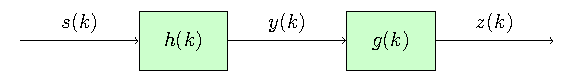
\includegraphics[width=\linewidth]{figures/example_fig.pdf}
            \end{figure}
        }
        \only<4-4>{
            \begin{theorem}
                \lipsum[1][1]\manualcite{10}{jiang2024terahertz}
            \end{theorem}
        }
    \end{columns}

    \only<5->{
        \vspace{0.5cm}
        \lipsum[1][1-5] \\
        \lipsum[1][1-3]
    }
\end{frame}

%@@@@@@@@@@@@@@@@@@@@@@@@@@@@@@@@@@@@@@@@@@@@@@@@@@@@@
\subsection{First subsection}

%-----------------------------------------------------
\begin{frame}[t, label=equations]
\frametitle{Equation, itemize, and enumerate}

    \begin{enumerate}
        \item A normal equation:
        \begin{equation}
            E = mc^2
        \end{equation}
        \begin{enumerate}
            \item level 1.1
            \begin{enumerate}
                \item level 1.1.1
                \item level 1.1.2
            \end{enumerate}
        \end{enumerate}
    \end{enumerate}
    
    \begin{itemize}
        \item Equation with tcbox:
        \begin{center}
            \tcboxmath{
                E = mc^2
            }
        \end{center}
        \begin{itemize}
            \item level 1.1
            \begin{itemize}
                \item level 1.1.1
            \end{itemize}
        \end{itemize}
    \end{itemize}
\end{frame}

%@@@@@@@@@@@@@@@@@@@@@@@@@@@@@@@@@@@@@@@@@@@@@@@@@@@@@
\subsection{Second subsection}

%-----------------------------------------------------
\begin{frame}[t, label=blocktheme]
\frametitle{Block themes}

    \begin{block}{Basic block}
        \begin{itemize}
            \item \lipsum[1][1-2]
        \end{itemize}
    \end{block}
    
    \begin{alertblock}{Alert block}
        \begin{itemize}
            \item \lipsum[1][1-1]\cite{belghazi2018mutual}.
        \end{itemize}
    \end{alertblock}

    \begin{exampleblock}{Example block}
        \begin{enumerate}
            \item \lipsum[1][1-3]\cite{berisha2014empirical}.
        \end{enumerate}
    \end{exampleblock}
\end{frame}

%#####################################################
\section{Second section}

%-----------------------------------------------------
\begin{frame}[t, label=tikzfigure]
\frametitle{Tikz figure}
    \begin{itemize}
        \item An example\manualcite{28}{Thesis2023}:
    \end{itemize}
    
    \begin{center}
        \includestandalone[scale=.7]{./figures/example_tikz}
    \end{center}
\end{frame}

%-----------------------------------------------------
\begin{frame}[plain, label=thank] % plain option removes footline
    \hspace*{-0.45cm}
    \begin{tikzpicture}[remember picture]
        % Top-left pattern
        \node[anchor=north west, inner sep=0pt, outer sep=0pt] 
        at (current page.north west) {
\includegraphics[width=2cm]{footages/top-left-pattern.png}};
        
        % Top-right pattern
        \node[anchor=north east, inner sep=0pt, outer sep=0pt] 
        at (current page.north east) {
\includegraphics[width=2cm]{footages/top-right-pattern.png}};
        
        % Bottom-left pattern
        \node[anchor=south west, inner sep=0pt, outer sep=0pt] 
        at (current page.south west) {
\includegraphics[width=2cm]{footages/bottom-left-pattern.png}};
        
        % Bottom-right pattern
        \node[anchor=south east, inner sep=0pt, outer sep=0pt] 
        at (current page.south east) {
\includegraphics[width=2cm]{footages/bottom-right-pattern.png}};
        
        % Centered Text (Main Message)
        \node[anchor=center] at (current page.center) {
            \begin{minipage}{0.8\textwidth}
                \centering
                {\color{primary} \Huge \textbf{Thanks for your attention!}}
                \vspace{1cm}
                
                \raggedright
                \hspace{2cm} \huge \textbf{Any questions?} \\
                \hspace{2cm} \Large You can find me at \\[0.5em] 
                \hspace{2cm} \checkmark \color{red!80!black}\texttt{email@domain.com}
            \end{minipage}
        };
    \end{tikzpicture}
\end{frame}

\end{document}